\subsection{Разработка моделей представления системы}
\label{sec:develop:umlDiagrams}

\subsubsection{} Диаграмма вариантов использования
\label{sec:develop:umlDiagrams:useCase}

Диаграмма вариантов использования наглядно показывает взаимодействия актеров с системой. Диаграмма вариантов использования показывает, какая функциональность реализуется в системе, основные функции, которые включены в систему (use case), их окружение (actors) и взаимодействие функций с окружением.

~
\begin{figure}[H]
\centering
	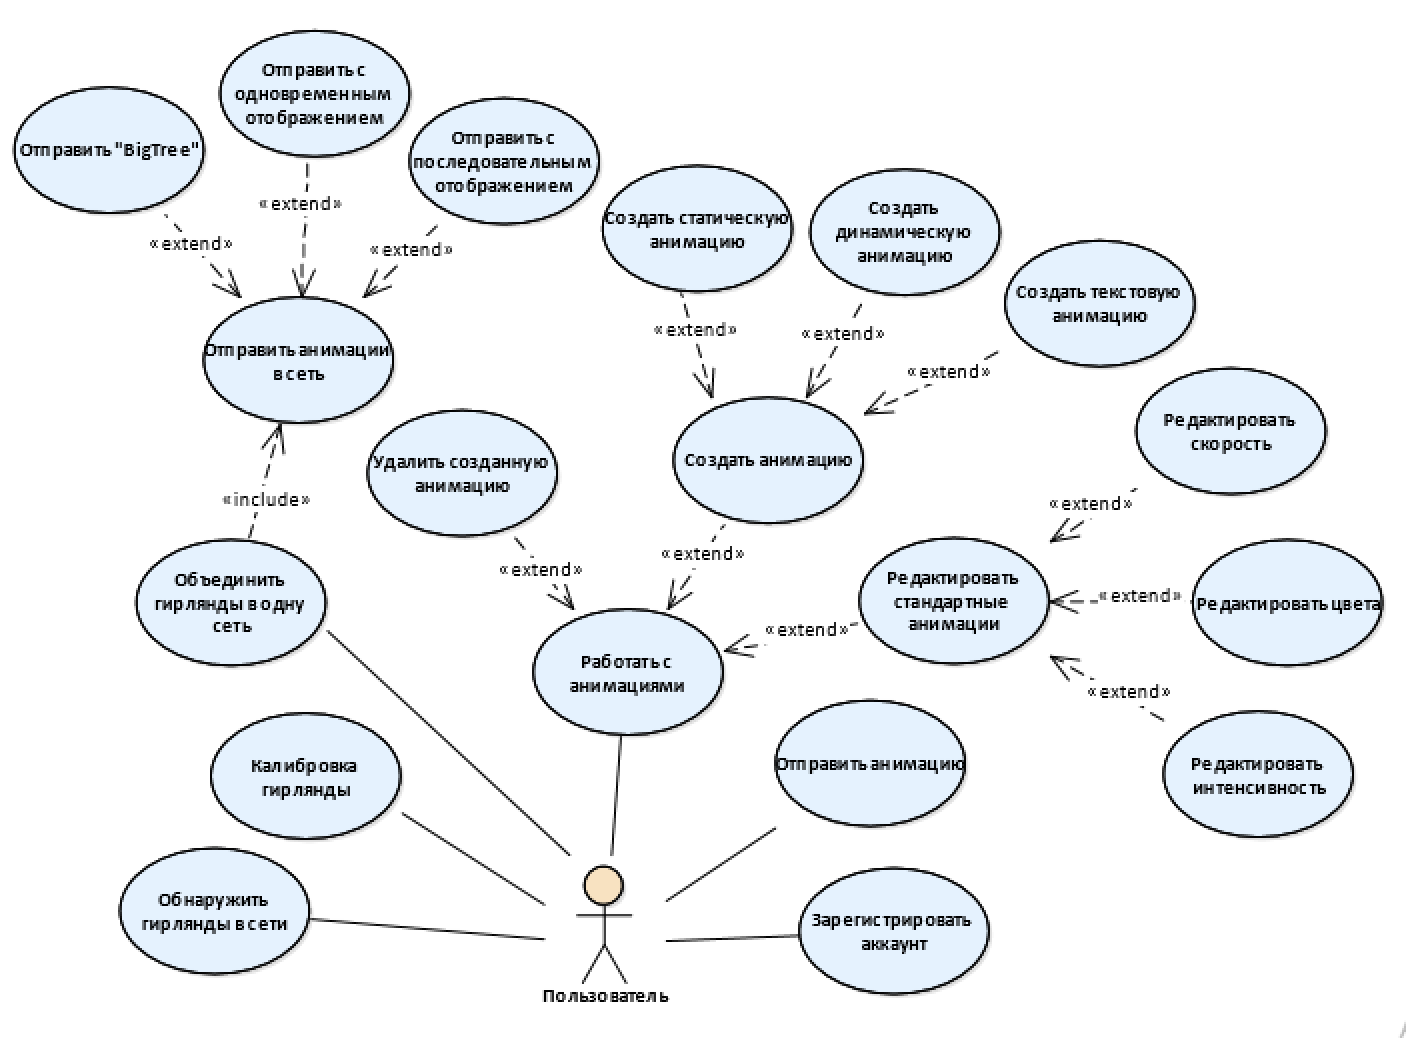
\includegraphics[scale=0.65]{figures/diagrams/uml_useCase.png}
	\caption{Диаграмма использования системы}
	\label{fig:develop:umlDiagrams:useCase}
\end{figure}

\subsubsection{} Диаграмма последовательности
\label{sec:develop:umlDiagrams:sequence}

На диаграмме последовательностей могут присутствовать участники процесса (пользователь и адресная светодиодная лента), компоненты системы, и сообщения, которые они могут вернуть. После запуска приложения оно пытается автоматически подключится к адресной светодиодной ленте. После успешного подключения пользователь может начать редактировать стандартные анимации, постоянно перезаписывая их в базе данных. Если пользователь захочет отправить анимацию на адресную ленту, то приложение возьмет ее из базы данных, конвертирует в байты (чтобы лента могла ее воспроизвести), отчистит адресную ленту от текущей анимации на ней и отправит ее по TCP сокетам. Данная диаграмма отражена в приложении Б.

\subsubsection{} Диаграмма компонентов
\label{sec:develop:umlDiagrams:component}

Диаграмма компонентов позволяет определить архитектуру разрабатываемой системы, установив зависимости между программными компонентами, в роли которых может выступать исходный  и исполняемый код. Диаграмму можно увидеть на рисунке~\ref{fig:develop:umlDiagrams:component}.

~
\begin{figure}[H]
\centering
	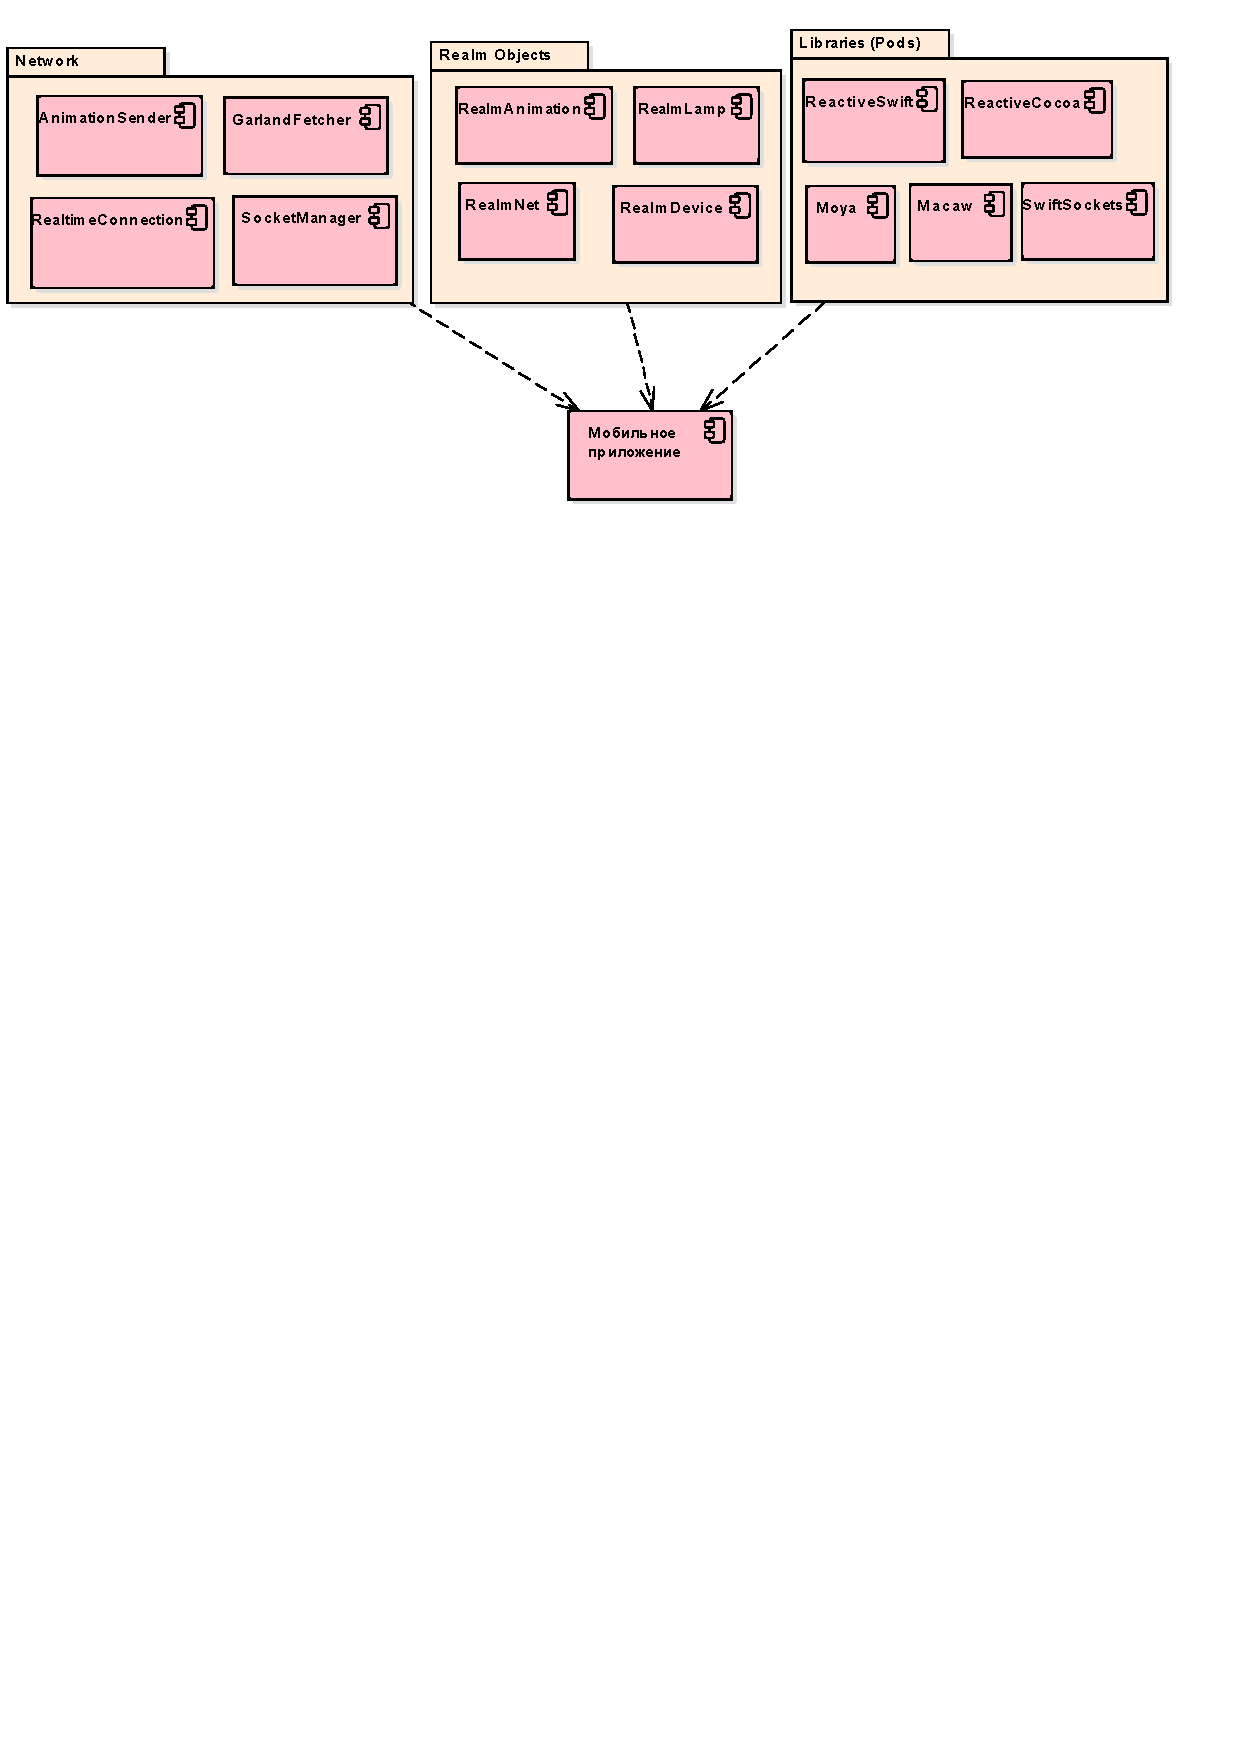
\includegraphics[scale=0.8]{figures/diagrams/uml_component.pdf}
	\caption{Диаграмма компонентов системы для управления световым оборудованием}
	\label{fig:develop:umlDiagrams:component}
\end{figure}

\subsubsection{} Диаграмма развертывания
\label{sec:develop:umlDiagrams:deployment}

Диаграмма развертывания необходима для представления того, какие устройства будут использовать те или иные компоненты. Из диаграммы понятно, что для использования данного продукта, пользователь должен иметь мобильный телефон под управлением операционной системы iOS (iPhone), а также адресную светодиодную ленту. Для использования сетевых функций (через Firebase) нужно стабильное подключение к интернету (Рисунок~\ref{fig:develop:umlDiagrams:deployment}).

~
\begin{figure}[H]
\centering
	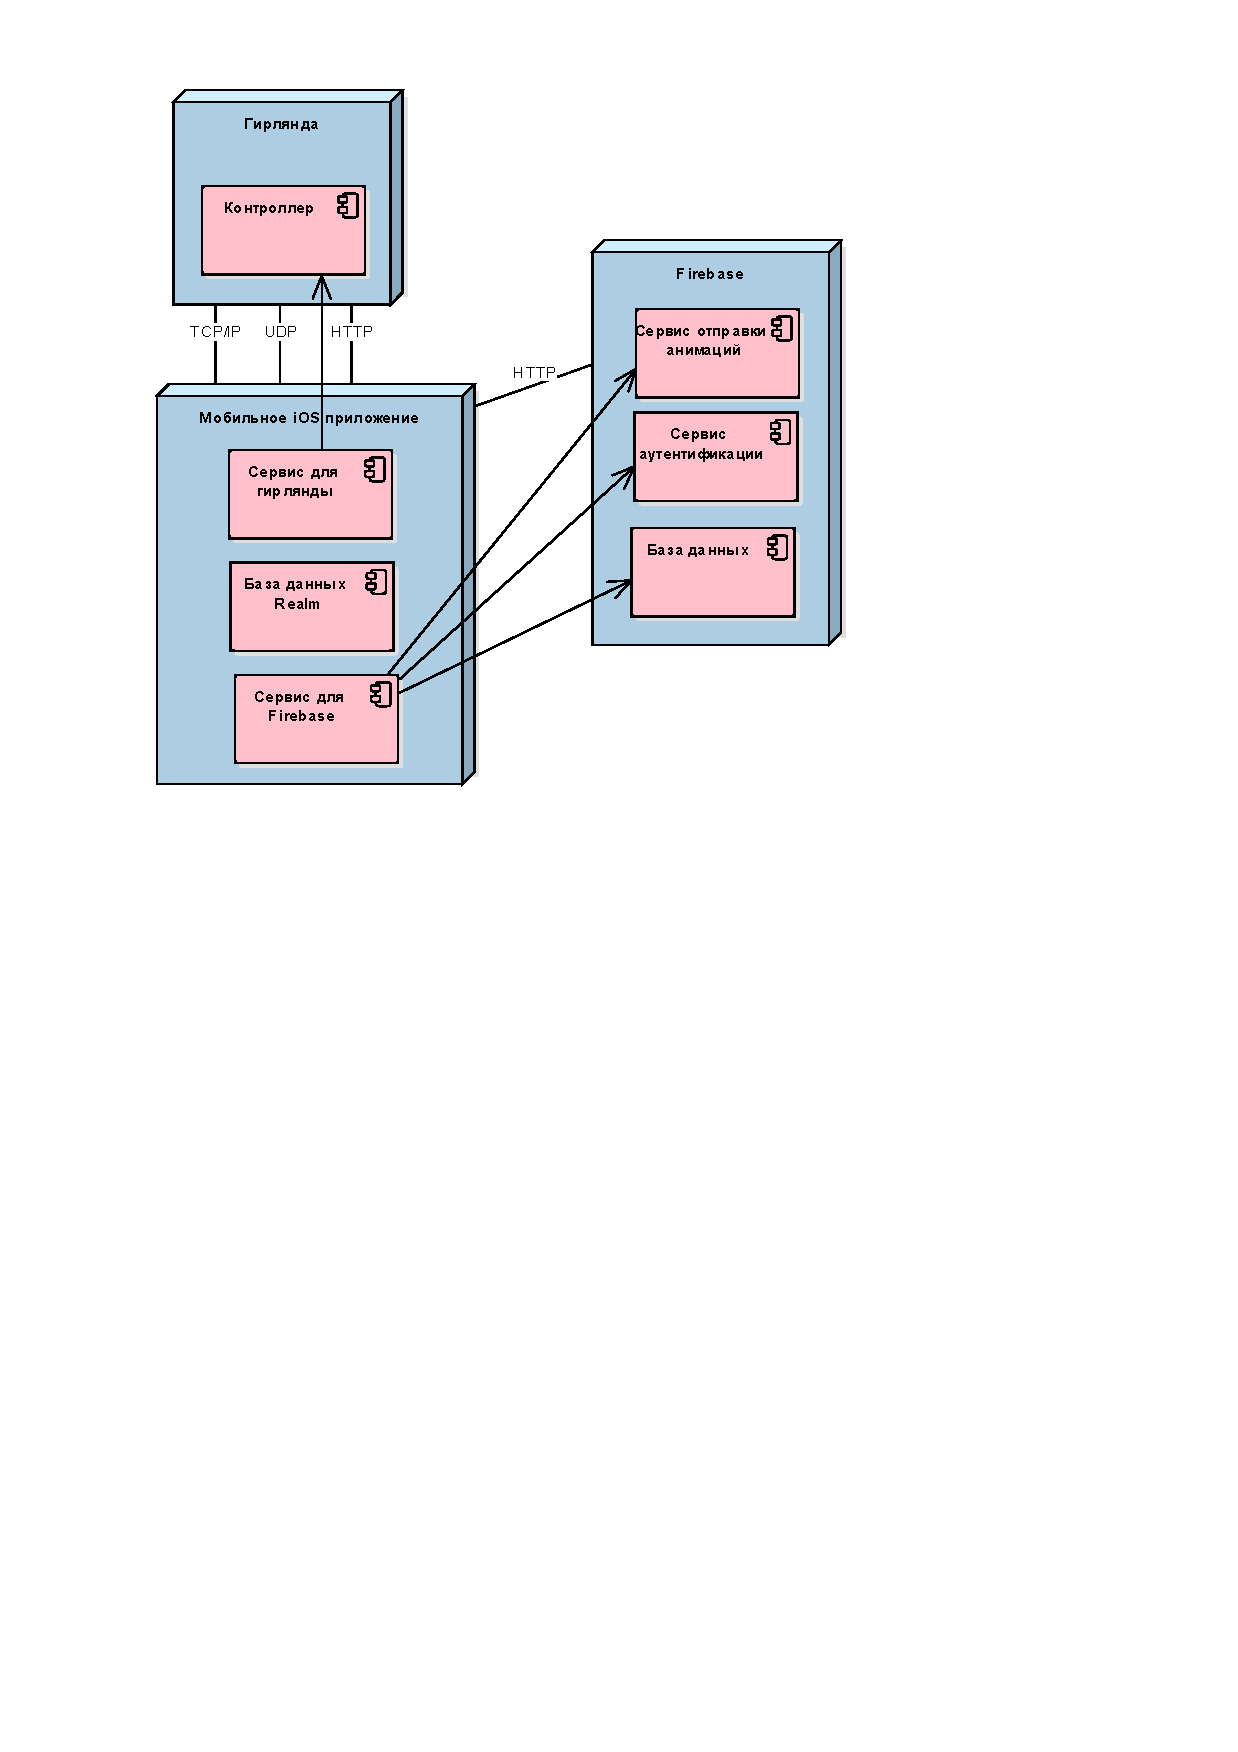
\includegraphics[scale=0.8]{figures/diagrams/uml_deployment.pdf}
	\caption{Диаграмма системы для управления световым оборудованием}
	\label{fig:develop:umlDiagrams:deployment}
\end{figure}

\subsubsection{} Диаграмма состояний
\label{sec:develop:umlDiagrams:useCase}

Диаграмма состояний описывает все возможные состояния процесса отправки анимации. На данной диаграмме показаны все возможные состояния, которые может принимать анимация. Если адресная светодиодная лента многоканальная, то перед отправкой ее надо расширить на нужное количество лампочек. При отправке анимации сначала посылается ее полное время проигрывания, потом адресная лента отчищается от уже воспроизводимой анимации, после идет конвертация данных анимации в байты и их последующая отправка по сокетам (Рисунок~\ref{fig:develop:umlDiagrams:state}).

~
\begin{figure}[H]
\centering
	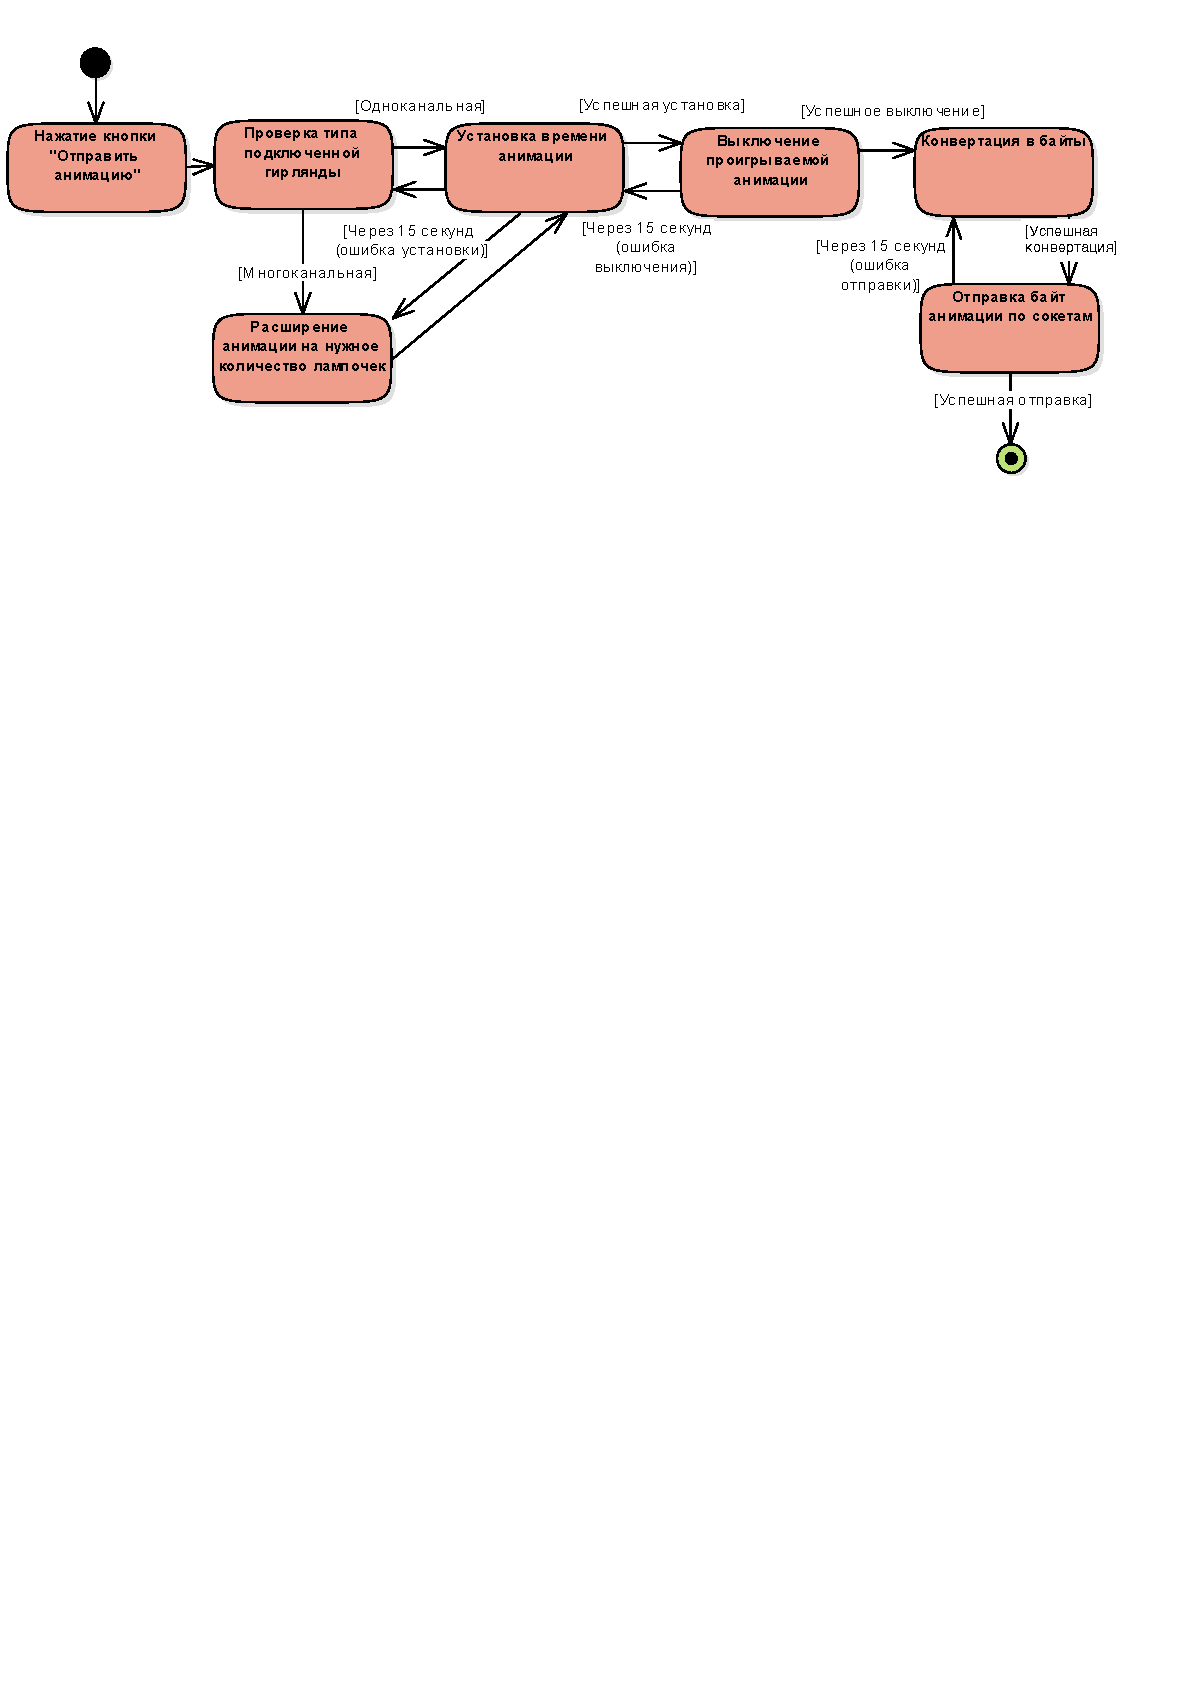
\includegraphics[scale=0.9]{figures/diagrams/uml_state.pdf}
	\caption{Диаграмма состояний анимации}
	\label{fig:develop:umlDiagrams:state}
\end{figure}

\subsubsection{} Диаграмма классов
\label{sec:develop:umlDiagrams:class}

Диаграмма классов используется для визуального изображения отношений между классами и интерфейсами в программе. Основными классами в данном проекте являются анимации, сервисы для работы с адресными светодиодными лентами, так же используются классы, реализующие паттерн MVC, контроллеры отображения и модели представления системы (view controllers, view models). В приложении А изображена диаграмма классов приложения.
